\chapter{Grundlagen und Methoden} 
In diesem Abschnitt werden die verwendeten Grundlagen und Methoden, die für die Umsetzung dieses Diplomarbeitsprojekts notwendig sind, dargestellt. Falls bei der Umsetzung mehrere Möglichkeiten zur Wahl standen, werden die einzelnen Möglichkeiten miteinander verglichen und nach einem Vergleich wird die besser geeignete Variante ausgewählt.


\section{Analyse des vorhandenen Systems}
Das bestehende System des Auftraggebers umfasst die Komponenten Grafana Server, Webserver und eine Datenbank mitsamt den notwendigen Algorithmen, um diese mit Echtzeitdaten zu befüllen. Bei der vorgegebenen Datenbank handelt es sich um einen MariaDB SQL-Server in der Version 10.1.48. Bei MySQL handelt es sich um eine quelloffene Implementierung des SQL Standards in der Version 5.0.12. In der nachfolgende Abbildung ist das vorhandene System des Auftraggebers ersichtlich.
\newline

\begin{figure}[h]
	\centering
	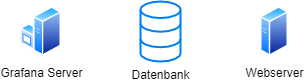
\includegraphics[height=3cm,width=10cm]{images/vorhandeneSystemAuftraggeber}
	\caption{vorhandeneSystemAuftraggeber}
	\label{fig:vorhandeneSystemAuftraggeber}
\end{figure}
Der Grafana Server wird übernommen, um Dashboards für die Energiesysteme und Panels für die Energietechnologien zu erstellen. Dabei können mehrere Statistiken, auch Panels genannt, zu einem Dashboard zusammengefasst werden, um somit eine Ordnerstruktur am Grafana Server zu erlangen. Der Webserver wird als Produktivserver benützt, um die fertige Website zu präsentieren. Die vorhandene Datenbank wird aufgrund deren Schemas nicht übernommen, stattdessen wird ein neues besseres Datenbankschema entwickelt. Die dafür notwendigen Algorithmen, um die neue Datenbank mit Echtzeitdaten zu befüllen, werden vom Auftraggeber entwickelt.



\subsection{Begriffe}
In diesem Abschnitt werden notwendige Begriffe, die in dieser Diplomarbeit eine wichtige Rolle spielen und zu Missverständnissen führen könnten, erklärt.

\subsubsection{Echtzeitdaten} \label{sec:Echtzeitdaten}
Der Begriff Echtzeitdaten ist definiert durch die regelmäßige und in gleichen Zeitabständen erfolgende Erfassung sowie Verarbeitung von Daten einer Energietechnologie. Der Zeitabstand der Datenerfassung bei den Energietechnologien beträgt 30 Sekunden. Aufgrund des vorgegebenen Zeitabstandes werden die Echtzeitdaten als weiche Echtzeitanforderung definiert, da das Produkt alle einkommenden Daten schnellstmöglich mit einem konstanten Zeitabstand von 30 Sekunden bearbeitet. Ein Überschreiten dieser Zeitgrenze wird nicht als Versagen definiert, solange sich die Zeit noch in einem akzeptablen Toleranzbereich von wenigen Sekunden befindet. Eine Unterschreitung der Zeitangabe ist sehr selten möglich.  


\subsubsection{Energietechnologie} \label{sec:Energietechnologie}
Als Energietechnologie wird ein Stromerzeuger, Stromverbraucher oder ein Energiespeicher bezeichnet. Stromerzeuger sind PV-Anlagen oder Windkraftanlagen. Stromverbraucher sind E-Ladestationen oder Hausanschlusszähler. Batteriespeicher oder Wärmespeicher sind Speicher-Energietechnologien. Die von diesen Technologien erfassten Echtzeitdaten werden in einer Datenbank gespeichert und anschließend grafisch in Form von Statistiken visualisiert.

Dabei werden folgende Echtzeitdaten für die Statistiken verwendet:

\begin{itemize}
	\item Erzeuger/Verbraucher - Leistung [kW]
	\item Erzeuger/Verbraucher - Energie [kW/h]
	\item Speicher – Kapazität/Temperatur [kW/h]/[°]
\end{itemize}

Die folgende Tabelle bietet eine Übersicht aller vorhandenen Energietechnologien.
In der ersten Spalte der Tabelle befinden sich reine Erzeuger-Energietechnologien[PM1] . Verbraucher-Energietechnologien sind in der zweiten Spalte ersichtlich. Speicher-Energietechnologien in der dritten Spalte und in der vierten und zugleich auch letzten Spalte befinden sich Energietechnologien, die sowohl als Verbraucher-Energietechnologie und als Erzeuger-Energietechnologie definiert sind.
\begin{table}[]
	\begin{tabular}{|l|l|l|l|}
		\hline
		\textbf{Erzeuger} &\textbf{Verbraucher}  & 	\textbf{Speicher}            &  \textbf{Verbraucher \& Erzeuger}           \\ \hline
		PV-Anlage                   & Wasserstoff- Elektrolyse    & Batteriespeicher     & Biomasseheizkraftwerk             \\ \hline
		Stromnetzbezug              & E-Ladestation               & Wasserstoff-speicher & Biomasseheizwerk                  \\ \hline
		Wasserstoff Brennstoffzelle & Hausanschlusszähler         & Wärmespeicher        & Biomassekessel                    \\ \hline
		Windkraftanlage             & Gebäude- Wärmebedarfszähler & Kältespeicher        & Kompressionskältemaschine         \\ \hline
		Wärmenetzbezug              & Gebäude- Kältebedarfszähler &                      & Ab- oder \newline \\ &&&Adsorptionskältemaschine \\ \hline
		Solarthermieanlage          &                             &                      &                                   \\ \hline
		Wärmepumpe                  &                             &                      &                                   \\ \hline
	\end{tabular}
\caption{Energietechnologien}
\label{tab:Energietechnologien}
\end{table}


\newpage
\subsubsection{Energiesystem} \label{sec:Energiesystem}
Der Begriff Energiesystem fasst mehrere Energietechnologien in einem bestimmten Gebiet, die genau einem Energiesystem zugeordnet sind, logisch zusammen. Ein Energiesystem kann somit eine Gemeinde, ein Gebäude oder ein einziger Haushalt mit mehreren Energietechnologien sein.


\subsubsection{Front-End} \label{sec:Front-End}
Der Begriff Front-End beschreibt die Weboberfläche auf welcher der Benutzer verschiedene Interaktionen durchführen kann. Dabei umfasst dieser Begriff alle Unterseiten der Weboberfläche welche von einem Benutzer verwendet werden können.


\subsubsection{Back-End} \label{sec:Back-End}
Mit dem Begriff Back-End ist das Laravel-Projekt, welches für die Ereignisse der Benutzer-Interaktionen zuständig ist, gemeint. Zusätzlich sind in diesem Begriff die Zugriffe auf die Datenbank sowie auf den Grafana Server mit eingebunden, welche durch das Laravel-Projekt durchgeführt werden.

\section{Anforderungen an das Produkt}
Die Datenbank des Auftraggebers ist die größte Schwachstelle des vorhanden Systems.
Aufgrund dessen wird ein neues Datenbankschema entwickelt. Neben der Entwicklung eines neuen Datenbankschemas sind folgende Anforderungen an das Produkt gegeben:

\begin{itemize}
	\item Übersichtliche Darstellung von Energiesystemen und Energietechnologien auf einem Kartendienst
	\item Grafana-Statistiken mit Echtzeitdaten der Energietechnologien anzeigen
	\item Bildergalerie um Energietechnologien eines ausgewählten Energiesystems zu präsentieren
	\item Managementfunktion mit Hilfe von verschiedenen Benutzern für unterschiedliche Berechtigungen
\end{itemize}


\subsection{Schutz von vertraulichen Informationen}
Sämtliche Daten wie Adressen, Standorte (in Form von Koordinaten) oder die Namen der Ersteller von Energiesystemen oder Energietechnologien sind vertrauliche Informationen und sollten somit nicht für jeden einsehbar sein. Darum sind diese Daten nur in der Datenbank gespeichert, welche nur für Benutzer mit entsprechender Berechtigung zugänglich ist. Die Daten, die in den Grafana-Statistiken dargestellt werden, sind ebenso vertrauliche Daten. Die Informationen, die man einer solchen Statistik entnehmen kann, könnten in die falschen Hände gelangen und zu unerwünschten Tätigkeiten führen. Um dieses zu verhindern, sieht jeder angemeldete Benutzer nur seine eigenen Statistiken und keine anderen. Ein nicht angemeldeter Besucher sieht keine Statistiken.


\subsection{Statistische Auswertung}
Text



\section{Architektur des Zielsystems}
Die \autoref{fig:Architektur} repräsentiert die Architektur des Zielsystems. Der Benutzer greift über die Weboberfläche auf den Webserver zu, wo sich das Laravel-Projekt befindet. Auf dieser Website kann der Benutzer verschiedene Interaktionen durchführen. Dabei ist die Weboberfläche ständig in Verbindung mit der Datenbank sowie dem Grafana Server. Sobald der Benutzer auf die Energiesysteme-Seite der Weboberfläche wechselt, wird eine Datenbankabfrage aller vorhandenen Energiesysteme durchgeführt. Zusätzlich dazu wird mittels API-Abfrage auf den Grafana Server zugegriffen, um Statistiken einer Energietechnologie anzuzeigen, falls dies vom Benutzer angefordert wird.

\begin{figure}[h]
	\centering
	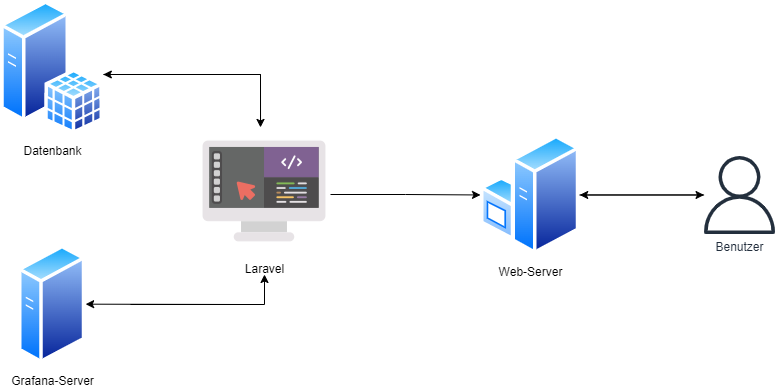
\includegraphics[height=8cm,width=15cm]{images/Architektur}
	\caption{Architektur}
	\label{fig:Architektur}
\end{figure}

\subsection{Endgeräte}
Text

\subsection{Serverseitig}
Text

\subsection{Clientseitige Interaktion des Benutzers}
Bei dem Punkt Clientseitig befindet man sich in der Architektur des Zielsystems bei dem Element JavaScript und mit den damit verbundenen Interaktionen des Benutzers. Map-Interaktionen sind Interaktionen mit einer Karte, dazu gehört das Erstellen, Bearbeiten und Löschen von Energiesystemen sowie Energietechnologien. Eine weitere Interaktion wäre die Verwendung des Adresssuchfeldes, welche mit einem Klick auf den Button „Suche“ oder durch Drücken der Enter-Taste durchgeführt wird. Tabellen-Interaktionen sind eine zusätzliche clientseitige Aktion, da die vom DataTable\footnote{Eine genaue Begriffserklärung befindet sich in \ref{sec:DataTable}} bereitgestellten Funktionen wie die Suchfunktion, Sortierfunktion oder Seitennummerierung allesamt clientseitig stattfinden und somit keinen Einfluss auf das Back-End haben.
Folgende Abbildung zeigt den Aufbau der einzelnen Elemente, die zusammenarbeiten, um die Website zu erstellen.


\begin{figure}[h]
	\centering
	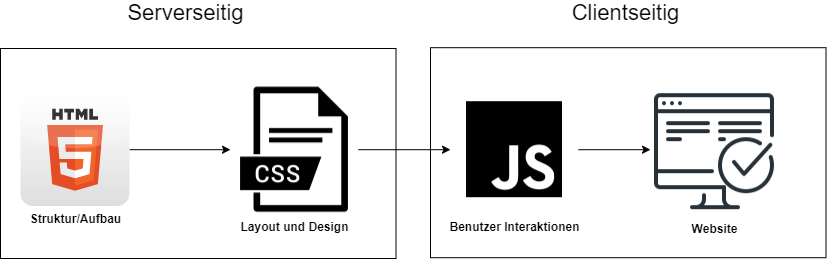
\includegraphics[height=4cm,width=12cm]{images/clientseitig}
	\caption{clientseitig}
	\label{fig:clientseitig}
\end{figure}

\subsection{Framework}
Die Wahl des Frameworks ist für die Umsetzung des Projekts entscheidend. Unter dem Begriff Framework versteht man eine Art Programmiergerüst, die es dem Programmierer deutlich erleichtert, ein Produkt zu erstellen. Jedes Framework bietet spezielle Lösungen und Lösungsansätze an und damit hat jedes einzelne sein eigenes Einsatzgebiet. In den nachfolgenden Unterkapiteln werden mögliche Frameworks für die Umsetzung des Projekts kurz erklärt. In \ref{sec:Entscheidung des Frameworks} wird genauer darauf eingegangen, welches Framework gewählt wurde und aus welchem Grund.

\subsubsection{Laravel}
Das PHP-Framework Laravel, welches 2011 entwickelt wurde, basiert auf dem MVC Muster\footnote{wird in  \autoref{sec:MVC} genauer erläutert} und bietet damit eine sehr gute Strukturierung und Übersicht beim Arbeiten. Laravel wird in den meisten Fällen als Back-End Framework verwendet. Die meisten Projekte werden mit Laravel im Back-End in Kombination mit Vue.js im Front-End umgesetzt. Genauere Informationen  zu Vue.js sind im Kapitel 2.6.3 nachzulesen. Laravel bietet jedoch die Möglichkeit, im Back- als auch im Front-End verwendet zu werden. Es lässt sich in folgende Einzelteile strukturieren:

\begin{itemize}
	\item Migrations 
	\item Views
	\item Controller 
	\item Models
	\item Routen 
\end{itemize}

Migrations sind die Abbildung der Tabellenstruktur und ermöglichen es, bei richtiger .env Datei Konfiguration, mit artisan Befehlen, ganz einfach eine Datenbank und die dazugehörigen Tabellen zu erstellen und diese auch genauso einfach wieder zu löschen oder zu leeren. Views fungieren als visueller Gliederungspart zwischen den Controllern und den Benutzern. In ihnen wird alles, was auf der Oberfläche ersichtlich ist, ausprogrammiert und gestaltet. Controller bilden die Verbindung zwischen den Views und den Models und ermöglichen es dem Benutzer, Daten mithilfe eines Zugriffs auf das Models zu verändern. Models bilden die Datenstruktur ab und ermöglichen den Zugriff auf die Daten und die Änderung dieser. Routen vermitteln die Benutzerabfrage von der View mit dem dazugehörigen Controller und werden in der Datei “web.php” definiert. Der ganze Prozess ist in \autoref{fig:Laravel MVC} visuell dargestellt. 
\begin{figure}[h]
	\centering
	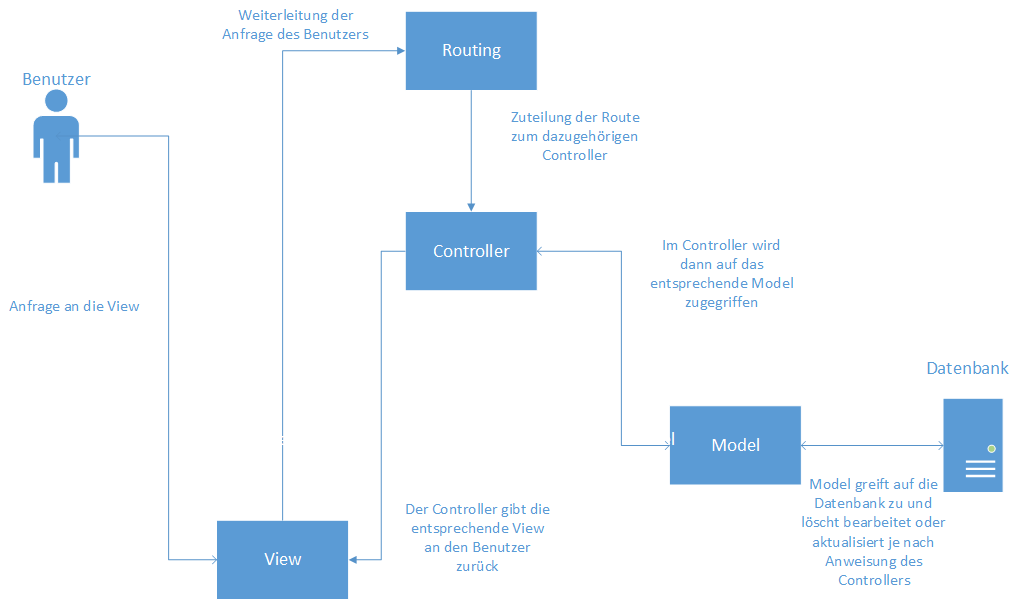
\includegraphics[height=8cm,width=15cm]{images/LaravelMVC}
	\caption{Laravel MVC}
	\label{fig:Laravel MVC}
\end{figure}
\subsubsection{Angular}
\subsubsection{ASP.NET}
\subsubsection{React}
\subsubsection{Entscheidung des Frameworks}\label{sec:Entscheidung des Frameworks}

\newpage
\subsection{Front-End Templates}
Die Auswahl des Front-End Templates ist essenziell für die Umsetzung der Weboberfläche des Produktes. Jedes Front-End Template bringt seine Vor- und Nachteile mit sich, wobei das Projektteam die Anforderungen an das Front-End Template mit den Vor- und Nachteilen jeden einzelnen Front-End Templates verglichen hat, um sich schlussendlich für eines zu entscheiden. Dabei sind die Anforderungen des Projektteams an das Front-End Template, dass es unkompliziert in das Projekt einzubinden ist und das Projektteam bereits Erfahrung damit hat, um das Arbeiten damit zu erleichtern. Weitere Anforderungen sind, dass es Responsive-Layouts ermöglicht, sowie Vorlagen von Komponenten, die eingebunden werden können, zur Verfügung stellt. Die drei Front-End Templates, die das Projektteam zur Auswahl stellt, sind Bootstrap, Tailwind und Vue.js.

\subsubsection{Bootstrap}
Bootstrap ist ein Open Source Front-End-CSS-Framework. Es basiert auf den Programmiersprachen HTML, CSS sowie JavaScript und stellt Gestaltungsvorlagen wie Formulare, Tabellen, Buttons und weitere Oberflächengestaltungen bereit. Bootstrap ist weltweit eines der bekanntesten und beliebtesten Front-End-Frameworks. Ebenso bietet Bootstrap eine Open Source-SVG-Icon-Bibliothek an, womit die Kompatibilität zwischen Komponenten und Icons bestenfalls gegeben ist. Vorteil dieses Templates ist, dass es leichtgewichtig ist, weil nur Front-End-Daten geladen werden müssen und keine Backend-Funktionalitäten. Zusätzlich ist es problemlos in das Projekt einzubinden und stellt mehrere Vorlagen zur Verfügung, die ebenso eingebunden werden können. Bootstrap ist kostenfrei zu verwenden, und das Projektteam bringt bereits Erfahrung mit diesem Template mit. Die Nachteile sind, dass Bootstrap wenige Back-End-Funktionen bereitstellt, und es ist weniger gut geeignet für sehr große Applikationen.

\subsubsection{Tailwind.css}
Tailwind ist ein Utility-First CSS-Framework, welches derzeit weltweit sehr beliebt ist. Diese Art von Framework soll mehr Flexibilität bieten als die traditionellen Vorgänger. Tailwind.css stellt Utility-Klassen zur Verfügung, mit denen man selbst Klassen zum Stylen der Komponenten definieren kann. Ein Inlinestylen ist bei diesem Framework ebenso möglich, womit externe CSS-Dateien überflüssig sind. Tailwind stellt Hilfsklassen zur Verfügung, welche das Arbeiten um einiges erleichtern. Zusätzlich bietet dieses Template eine hohe Flexibilität sowie mehrere Funktionen, um ein Responsive Design zu erreichen. Jedoch hat dieses Template keine vorgefertigten Komponenten, auf welche zurückgegriffen werden kann, und der Benutzer dieses Templates braucht sehr viel Zeit zum Erlernen der richtigen Verwendung. Die Größe der zu installierenden CSS-Datei ist sehr groß, da dieses Template eine breite Palette von Klassen bereitstellt, wobei die meisten oft in einem Projekt nicht verwendet werden. Das Projektteam hat mit diesem Template wenig Erfahrung, und die Dokumentation im Internet ist sehr mangelhaft.

\subsubsection{Vue.js}
Das JavaScript Framework Vue.js, welches für die Front-End-Entwicklung eingesetzt werden kann, wird immer populärer. Die Einfachheit und Benutzerfreundlichkeit ist ein Grund für die immer größer werdende Beliebtheit. Vue.js basiert auf dem virtuellen DOM \footnote{Virtuelles Document Object Model, beim Aktualisieren schneller als das herkömmliche}, was bedeutet, dass das Abarbeiten von Befehlen schneller funktioniert als beim herkömmlichen bekannten DOM\footnote{Document Object Model, stellt XML oder HTML Dokumente als Baumstruktur dar}. Vue.js basiert auf den Programmiersprachen HTML, CSS und JavaScript, womit die wichtigsten verwendeten Sprachen abgedeckt sind. Vue.js stellt Funktionen wie UniTests, End-to-End-Tests sowie Routing-Systeme bereit. Die Lesbarkeit bei diesem Template ist sehr gut, da alle Komponenten sich in einer Datei befinden. Das Projektteam hat nur wenig Erfahrung mit diesem Template und es herrschen generelle Sprachbarrieren, da vieles nur in der Sprache Chinesisch vorhanden ist.


\subsubsection{Entscheidung des Front-End Templates}
Das Projektteam hat sich für das Front-End Template Bootstrap CSS entschieden aufgrund der Vorteile, die es mit sich bringt. Diese Entscheidung wurde unter anderem deswegen so getroffen, da das Projektteam bereits Erfahrung mit diesem Framework sammeln konnte und dieses Framework alle Anforderungen, die an das Front-End Template gestellt wurden, erfüllt.
In der nachfolgenden Tabelle ist eine Gegenüberstellung der Vor- und Nachteile der Front-End Templates ersichtlich:

\begin{table}[h]
	\begin{tabular}{|l|l|l|}
		\hline
		\textbf{Front-End Template} &\textbf{Vorteile}  & 	\textbf{Nachteile}    \\ \hline
		
		\textbf{Bootstrap}                   &
		
		basiert auf HTML, CSS und JavaScript & wenige Back-End Funktionen \\ 
		&
		stellt Gestaltungsvorlagen bereit 
		&   nicht geeignet für große Applikationen \\
	 &	weltweit sehr bekannt und beliebt \\
		&
		leicht in das Projekt einzubinden \\
		&
		Projektteam hat bereits Erfahrungen damit
		
		
		
		          \\ \hline
		          
		\textbf{Tailwind.css}        &
		 
		weltweit sehr beliebt & keine vorgefertigten Komponenten \\
		&
		bietet mehr Flexibilität & Projektteam hat sehr wenig Erfahrung \\
		&
		stellt Utility-Klassen zur Verfügung &  		  Online-Dokumentation ist mangelhaft \\
		& &  		  erfahrungsloser Benutzer  \\
		&&  		  benötigt viel Einarbeitungszeit\\
		&&		  Größe der CSS-Datei ist enorm \\
	
		      \\ \hline
		      
		\textbf{Vue.js} &
		 einfach und benutzerfreundlich  & Projektteam hat wenig Erfahrung \\
		 &
		basiert auf HTML, CSS und JavaScript & 		 Sprachbarrieren, vieles nur auf Chinesisch \\
		&
		stellt Funktionen wie UniTests, \\
		&
		 End-to-End Tests und \\
		 &Routing-Systeme bereit \\
		 &
		hohe Lesbarkeit des Codes 
		
		                  \\ \hline
		                  
	\end{tabular}
	\caption{Vor- und Nachteile der Front-End Templates}
	\label{tab:Vor- und Nachteile der Front-End Templates}
\end{table}



\subsection{Verbindung der Datenbank mit Laravel}
\subsubsection{Laravel .env Datei }
\subsubsection{Migrations}
\subsubsection{Seeder / Factories}
\subsubsection{Datenübergabe in Laravel}


\section {Visuelle Darstellung der Energiesysteme und Energietechnologien }

\subsection{Kartendienste}

\subsubsection{Google Maps}
\subsubsection{OpenStreetMap}

\subsection{Geoinformationssystem }

\subsection{CSS-System}

\subsection{Auswahl des Anbieters}


\section{Berechtigungssystem Benutzer}
Im folgenden Abschnitt wird näher auf das Benutzerverwaltungssystem eingegangen sowie auf die vorhandenen Benutzerrollen, die einem Benutzer zugeteilt werden können.

\subsection{Benutzerrollen}
Die Weboberfläche bietet für deren Besucher ein rollenbasiertes Benutzersystem an, um die Funktionen für jeden Benutzer zu deklarieren.
Das rollenbasierte Benutzersystem unterscheidet zwischen folgenden Benutzern:

\begin{itemize}
	\item Administrator 
	\item Mitarbeiter
	\item Öffentlicher Benutzer 
\end{itemize}



\subsubsection{Administrator}
Der Administrator-Benutzer ist der höchste Benutzer von allen. Er darf Energiesysteme sowie Energietechnologien erstellen und alle anderen vorhandenen bearbeiten und löschen. Zusätzlich dazu hat er Einsicht in sämtliche Grafana-Statistiken. Diese Benutzerrolle hat das Recht, neue Benutzer auf der Weboberfläche zu registrieren und vorhandene zu löschen, was für alle anderen Benutzer nicht möglich ist.

\subsubsection{Mitarbeiter}
Die Rolle „Mitarbeiter“ darf auf der Weboberfläche neue Energiesysteme sowie Energietechnologien erstellen. Die von ihm erstellten Energiesysteme sowie Energietechnologien kann er bearbeiten oder  löschen, und er hat auf diesen ebenso die Berechtigung auf Einsicht der Statistiken. Andere Mitarbeiter dürfen seine Energiesysteme und Energietechnologien nicht bearbeiten oder löschen und haben keinen Zugriff auf dessen Statistiken mit Ausnahme des Administrators. Ein Mitarbeiter-Benutzer darf somit nur seine selbst erstellten Energiesysteme und Energietechnologien verwalten. Der Mitarbeiter-Benutzer hat nicht die Berechtigung, neue Benutzer zu registrieren oder vorhandene zu löschen.

\subsubsection{öffentlicher Benutzer}
Dieser Benutzer hat die geringste Berechtigung und tritt in Kraft, wenn man nicht auf der Weboberfläche angemeldet ist. Dieser Benutzer darf keine Energiesysteme sowie Energietechnologien erstellen, bearbeiten oder löschen. Zusätzlich hat der öffentliche Benutzer keine Einsicht auf sämtliche Grafana-Statistiken. Der Zugang zu der Benutzerverwaltung ist ebenso nicht erreichbar. Dieser Benutzer sieht lediglich die öffentlichen Daten, die für jedes Energiesystem und jede Energietechnologie preisgegeben werden.

\subsection{Berechtigungen in Laravel}
Im folgenden Abschnitt wird erklärt, wie in Laravel die zuvor genannten Benutzerrollen unterschieden werden.
Dafür bietet Laravel Authentifizierungsrichtlinien. Dabei kann mit den Befehlen @auth und @guest überprüft werden, ob der aktuelle Benutzer authentifiziert oder ein Gast ist. Je nach Authentifizierung und Rolle hat der Benutzer unterschiedliche Rechte sowie Funktionen zur Verfügung.
Für genauere Informationen, wie eine Berechtigungsüberprüfung in Laravel umgesetzt werden kann, siehe Quelle x.y.



\section{Ui/Ux Design}

\subsection{Wireframe}

\subsection{Persona}


\section{Template Layout}

\subsection{Platzhalter Yield}

\subsection{Sections}
\subsection{Einbindung der definierten Sections}


\section{Laravel Befehle}

\subsection{Migration Befehle}
\subsection{Seeder und Factory Befehle}
\subsection{Model und Controller Befehle}
\subsection{Starten des Laravel Develop Servers}
\subsection{Befehle nach dem Git Pull} 



\chapter{Ergebnisdokumentation }
Dieser Abschnitt beinhaltet eine Dokumentation der verwendeten Werkzeuge zur Umsetzung der einzelnen Funktionen. Es werden alle behandelten Teilbereiche erläutert.

\section{Laravel }
Text

\subsection{Installation}
Text

\subsection{Bootstrap Einbindung}
Text
\subsection{Grafana Einbindung}
Text

\subsection{MVC}\label{sec:MVC}
Text
\subsubsection{Model}
Text
\subsubsection{View}
Text
\subsubsection{Controller}
Text


\section{Datenbankanbindung in Laravel}
Text

\subsection{Datenbank Anmeldeinformationen}
Text

\subsection{Mail Server Konfigurationen}
Text

\subsection{Migrations}
Text


\section{Routen in Laravel}
Text

\subsection{Resource Routen}
Text

\subsection{GET Routen}
Text

\subsection{Auth Routen}
Text


\section{Datenbankdesign}
Text

\subsection{Erstellen eines neuen Schemas}
Text

\subsubsection{ER-Model}
Text

\subsubsection{Fremdschlüssel}
Text


\section{Corporate Design}
Text

\subsection{Vorschläge}
Text

\subsection{Änderungsvorschläge}
Text

\subsection{Finales Design}
Text

\subsection{Definierte Farben}
Text

\subsection{Überschriften}
Text

\subsection{Interaktionsfarben}
Text

\subsection{Schriftarten}
Text

\subsection{Schriftgrade}
Text

\subsection{Logo}
Text

\subsection{Verwendete Icons und deren Bedeutungen} \label{sec:Verwendete Icons und deren Bedeutungen}
Text

\subsection{Map Icons}
Text

\subsection{Icons in Formularen}
Text

\subsection{Icons im DataTable}
Text

\subsection{Buttons}
Text

\subsection{Tabelle mit generellen Informationen über einzelne HTML Elemente}
Text

\subsection{Datenformate}
Text



\section{Weboberfläche}
Im Abschnitt Weboberfläche wird speziell auf das Front-End sowie das Back-End des Produktes eingegangen. Bei dem Punkt Back-End vor allem auf die Funktionen, die für die Benutzer-Interaktionen zuständig sind, und bei dem Punkt Front-End auf das Layout sowie das Design der Weboberfläche.


\subsection{Backend}
In diesem Abschnitt wird genauer auf den Ablauf des Codes im Back-End, der für die Funktionen auf der Weboberfläche zuständig ist, eingegangen. 
Für jedes Energiesystem oder jede Energietechnologie stehen die Funktionen Erstellen, Bearbeiten und Löschen zur Verfügung. In den folgenden Abschnitten wird genauer auf diese Funktionen eingegangen.


\subsubsection{Energiesystem Erstellen}
Für das Erstellen eines Energiesystems ist ein Mausklick auf der Karte notwendig. Daraufhin öffnet sich ein Pop-up Fenster, um die Kerndaten des Energiesystems einzugeben.
Das Pop-up zum Erstellen eines Energiesystems ist in der Abbildung x.y ersichtlich.
Beim Erstellen eines Energiesystems werden folgende Attribute in der Datenbank erfasst:
Eingabe des Benutzers:
\begin{itemize}
	\item Bezeichnung 
	\item Katastralgemeinde
	\item Postleitzahl
\end{itemize}

Automatisch ausgefüllte Attribute, welche nicht im Pop-up dargestellt werden:
\begin{itemize}
	\item Längengrad 
	\item Breitengrad
	\item User-ID
\end{itemize}

Die Attribute Längengrad und Breitengrad werden automatisch mithilfe des Mausklicks auf der Karte mit den entsprechenden Koordinaten beim Erstellen des Energiesystems befüllt. Das Attribut User-ID wird automatisch mit der ID des gerade angemeldeten Benutzers ausgefüllt, um das Energiesystem einem Benutzer zuteilen zu können.
Nachdem der Benutzer alle Daten eingegeben hat, werden diese Daten an den Controller übermittelt, wo anschließend das Energiesystem erstellt und in der Datenbank erfasst wird. Als nächstes werden die gespeicherten Informationen wieder zurück an die Weboberfläche übergeben, um die Energiesysteme-Marker auf der Karte zu platzieren sowie den Inhalt der Liste aller vorhandenen Energiesysteme zu aktualisieren. Die folgende Abbildung zeigt den Ablauf, um ein Energiesystem zu erstellen:




\subsubsection{Energiesystem Bearbeiten}
Mit dem Stift-Icon beim Energiesystem in der Liste ist es möglich, die Kerndaten eines Energiesystems zu bearbeiten. Die zu bearbeitenden Daten, welche einen weißen Hintergrund  aufweisen, lauten auf „Bezeichnung“, „Katastralgemeinde“ und „Postleitzahl“. Die Koordinaten sowie die User-ID des Energiesystems bleiben konstant und sind nicht änderbar und nicht im Pop-up ersichtlich.
Folgende weitere Attribute werden bei jedem Energiesystem automatisch berechnet, angezeigt und sind nicht bearbeitbar, sondern dienen nur als weitere Information über das ausgewählte Energiesystem. Das Pop-up zum Bearbeiten eines Energiesystems ist in der Abbildung x.y ersichtlich.

\begin{itemize}
	\item Anzahl-Erzeugungstechnologien  
	\item Anzahl-Verbraucher
	\item Anzahl-Speicher
	\item Ges-Nennleistung [kW]
	\item Ges-Energie [kW/h]
	\item Ges-Verbraucher-Leistung [kW]
	\item Ges-Verbraucher-Energie [kW/h]
	\item Ges-Erzeuger-Leistung [kW]
	\item Ges-Erzeuger-Energie [kW/h]
	\item Ges-Speicher-Kapazität [kW/h]
	\item Aktueller Netzbezug [kW]
\end{itemize}

Für genauere Informationen zu den einzelnen Attributen siehe Kapitel  \ref{sec:Verwendete Icons und deren Bedeutungen}
Mit dem Button „Mehr Details zu diesem Energiesystem“ ist es möglich, die weiteren Daten des Energiesystems ein- und auszuklappen. 
Nachdem der Benutzer die Attribute des Energiesystems bearbeitet hat, werden diese mithilfe des Controllers in der Datenbank aktualisiert. Anschließend werden die neuen Daten der Weboberfläche übergeben, um auf der Karte sowie in der Liste den aktuellen Stand der Energiesysteme darstellen zu können. In der Abbildung x.y ist der Ablauf „Energiesystem bearbeiten“ dargestellt:



\subsubsection{Energiesystem Löschen}
Um ein Energiesystem zu löschen, benötigt man das Mülleimer-Icon, welches sich neben jedem Energiesystem in der Liste befindet, sofern der angemeldete Benutzer die erforderliche Berechtigung dazu hat. 
Nachdem dieses Icon betätigt wurde, wird die Information, dass ein Energiesystem gelöscht wurde, an den Controller übermittelt. Dieser löscht anschließend mithilfe der ID des ausgewählten Energiesystems dieses aus der Datenbank und übergibt alle anderen Energiesysteme zurück auf die Weboberfläche, um die vorhandenen Energiesysteme auf der Karte zu platzieren sowie in der Liste anzuzeigen. Der Ablauf, um ein Energiesystem zu löschen, wird in folgendem Diagramm präsentiert:



\subsubsection{Energietechnologie Erstellen}
Für das Erstellen einer Energietechnologie ist das Auswählen eines Energiesystems mit einem Doppelklick notwendig. Anschließend verwandelt sich der Cursor in das Energietechnologie-Icon, welches darauf hindeutet, dass jetzt das Hinzufügen einer Energietechnologie mittels eines Klicks auf der gewünschten Position auf der Karte möglich ist. Nach dem Klick auf der Karte öffnet sich ein Pop-up-Fenster, um die Kerndaten der Energietechnologie einzugeben. Dieses Pop-up ist in der Abbildung x.y ersichtlich. 

Eingabe des Benutzers:
\begin{itemize}
	\item Bezeichnung 
	\item Typ
	\item Ort
	\item Bild einfügen
	\item Beschreibung
\end{itemize}

Automatisch ausgefüllt und nicht im Pop-up dargestellt:
\begin{itemize}
	\item Längengrad 
	\item Breitengrad
	\item Ensys-ID
	\item User-ID
\end{itemize}

Nachdem der Benutzer die Daten im Pop-up ausgefüllt hat, werden diese Informationen über den Controller in der Datenbank erfasst. Anschließend werden die Energietechnologie-Daten an die Weboberfläche übermittelt, um die Energietechnologien auf der Karte darzustellen sowie in der Liste anzuzeigen. Der Ablauf, um eine Energietechnologie zu erstellen, wird in der Abbildung x.y dargestellt:


\subsubsection{Energietechnologie Bearbeiten}
Um eine Energietechnologie zu bearbeiten, muss zuerst ein Energiesystem mit einem Doppelklick ausgewählt werden. Anschließend befinden sich rechts in der Liste alle dazugehörigen Energietechnologien, welche man mit dem Stift-Icon bearbeiten kann. Nach dem Betätigen des Stift-Icons öffnet sich ein Pop-up-Fenster, um die Attribute zu bearbeiten. Dieses Pop-up-Fenster ist in der Abbildung x.y ersichtlich.
Dabei sind die Attribute „Bezeichnung“, „Ort“, „Bild“ und „Beschreibung“ bearbeitbar. Um dem Benutzer dies deutlich zu machen, weisen diese Attribute einen weißen Hintergrund auf. 
Die Attribute „Typ“, „Längengrad“, „Breitengrad“, „Ensys-ID“ sowie „User-ID“ sind nicht bearbeitbar.
Nachdem der Benutzer die Daten bearbeitet hat, werden diese über den Controller in die Datenbank geschrieben. Anschließend werden die Energietechnologie-Daten an die Weboberfläche übergeben, um die Marker auf der Karte zu platzieren sowie den Inhalt der Liste zu aktualisieren. Das nachfolgende Diagramm beschreibt den Ablauf für das Bearbeiten einer Energietechnologie:



\subsubsection{Energietechnologie Löschen}
Um eine Energietechnologie zu löschen, benötigt man das Mülleimer-Icon, welches sich in der Liste neben den Energietechnologien befindet, sofern ein Energiesystem von dem Benutzer ausgewählt wurde.
Sobald der Benutzer dieses Icon betätigt, wird mithilfe der ID der ausgewählten Energietechnologie dem Controller mitgeteilt, dass diese Energietechnologie gelöscht werden soll. Daraufhin löscht der Controller diese Energietechnologie aus der Datenbank und übergibt anschließend alle anderen vorhandenen Energietechnologie-Daten an die Weboberfläche, um dort die Marker zu platzieren sowie den Inhalt der Liste zu aktualisieren. Das nachfolgende Diagramm beschreibt den Ablauf für das Löschen einer Energietechnologie:



\subsubsection{Benutzerverwaltung}
Je nach Benutzerrolle des aktuell angemeldeten Benutzers stehen dem Benutzer unterschiedliche Funktionen auf der Weboberfläche zur Verfügung.  
Folgende drei Benutzer stehen zur Verfügung:
\begin{itemize}
	\item Administrator 
	\item Mitarbeiter
	\item Öffentlicher Benutzer
\end{itemize}
Wie eine generelle Überprüfung des Benutzers in Laravel umgesetzt werden kann, ist unter der Quelle x.y ersichtlich. Folgende Überprüfung wurde selbst vom Projektteam entwickelt und ist somit nicht unter der genannten Quelle auffindbar.
Mit folgender Überprüfung wird kontrolliert, ob der gerade angemeldete Benutzer das Energiesystem oder die Energietechnologie selbst erstellt hat oder ob er die Rolle des Administrators aufweisen kann. Falls der Benutzer das Energiesystem oder die Energietechnologie selbst erstellt hat, ist der erste Teil der Überprüfung erfüllt und der Benutzer hat die Verwaltungsfunktionen zur Verfügung. Falls der Benutzer das Energiesystem oder die Energietechnologie nicht selbst erstellt hat, wird die zweite Überprüfung durchgeführt, welche überprüft, ob der Benutzer die Rolle des Administrators aufweisen kann. Falls er diese Rolle besitzt, hat er die Verwaltungsfunktionen zur Verfügung, andernfalls nicht.


\subsubsection{Adresssuche}
Mithilfe des Adresssuchfeldes ist es möglich, einen Standort einzugeben, um anschließend auf der Karte zu diesem zu gelangen. Dadurch ist das Auffinden von bestimmten Orten auf der Karte problemlos möglich. Dabei wird die eingegebene Adresse in geografische Koordinaten umgewandelt, zu welchen man anschließend navigiert wird. In der folgenden Abbildung ist das Adresssuchfeld ersichtlich.

Folgende Schreibweisen sind in der Suche möglich:
\begin{itemize}
	\item Stadt 
	\item Land
	\item Straße 
	\item Postleitzahl 
\end{itemize}

\textbf{Automatische Vervollständigung} \\
Um die Suche nach der richtigen Adresse zu vereinfachen, wird die Eingabe des Benutzers mit einer Auto-Complete-Funktion unterstützt. Diese Funktion bietet mögliche Ziel-Adressen anhand der bisher eingegebenen Daten an, welche vom Benutzer ausgewählt werden können. Ein Beispiel dieser Funktion ist in der Abbildung x.y dargestellt. \\

\textbf{Adresssuche durchführen} \\
Die Adresssuche kann auf zwei verschiedene Arten durchgeführt werden.
Die erste Variante ist das Benutzen des dazugehörigen Buttons mit der Beschriftung „Suchen“. Die zweite Variante ist das Betätigen der Enter-Taste auf der Tastatur. Beide Varianten führen zu dem gleichen Ergebnis, und zwar, dass die Adresssuche durchgeführt wird.
Sobald die Adresssuche durchgeführt wird, werden für die eingegebene Adresse die dazugehörigen Koordinaten berechnet. Sobald diese berechnet wurden, werden diese an die Karte übergeben, damit der Mittelpunkt der Karte auf diese Koordinaten gesetzt wird. Anschließend gelangt der Benutzer zu seiner eingegebenen Adresse auf der Karte und kann seine Interaktionen fortsetzen. Das folgende Diagramm beschreibt die Durchführung der Adresssuche:



\subsection{Front-End}
Text

\subsubsection{Home}
Text

\subsubsection{Energiesysteme}
Text

\subsubsection{Galerie}
Text

\subsubsection{Impressum}
Text

\subsubsection{Datenschutz}
Text

\subsubsection{Registrierungsseite}
Text

\subsection{Login}
Text

\subsection{Registrierung}
Text

\subsection{Kartendienst Funktionalitäten}
Neben den bekannten Kartendienst-Funktionen wie das Erstellen eines Energiesystems oder einer Energietechnologie bietet die Karte weitere Funktionen. Diese weiteren Funktionen sind das Auswählen und Abwählen eines Energiesystems.

\subsubsection{Auswählen eines Energiesystems}
Das Auswählen eines Energiesystems ist notwendig, um die dazugehörigen Energietechnologien auf der Karte sowie in der Liste zu sehen. Ebenso ist es notwendig, um neue Energietechnologien erstellen zu können.
Mit einem einfachen Klick auf das Energiesystem-Icon wird an dieses Energiesystem lediglich herangezoomt, jedoch noch nicht ausgewählt.
Um ein Energiesystem auszuwählen, ist ein Doppelklick darauf notwendig. Dieser Doppelklick bewirkt, dass in der Liste sowie auf der Karte die dazugehörigen Energietechnologien angezeigt werden. Anschließend ist es für den Benutzer möglich, die Energietechnologien zu verwalten. Der Ablauf für das Auswählen eines Energiesystems wird in der folgenden Abbildung dargestellt:



\subsubsection{Abwählen eines Energiesystems}
Nachdem ein Energiesystem ausgewählt wurde, ist mit einem einfachen Linksklick auf das Energiesystem-Icon möglich, das ausgewählte Energiesystem wieder abzuwählen. Nach Abwählen des Energiesystems werden die dazugehörigen Technologien wieder von der Karte sowie aus der Tabelle entfernt. Stattdessen werden in der Tabelle wieder alle vorhandenen Energiesysteme angezeigt. Der Ablauf für das Abwählen eines Energiesystems wird in der folgenden Abbildung dargestellt.



\subsection{Anzeige von Energiesystemen und Energietechnologien auf der Karte}
In diesem Abschnitt werden die Funktionen zum Darstellen und Entfernen der Marker auf der Karte erläutert.



\subsubsection{Energiesysteme Marker auf der Karte platzieren}
Immer wenn die Map neu geladen wird, werden alle vorhandenen Energiesysteme in Form von Icons auf der Karte platziert. Dafür werden die Daten aller Energiesysteme aus der Datenbank gelesen, um anschließend die Marker auf der Karte platzieren zu können. Die dafür notwendigen Datenbank-Attribute, die ausgelesen werden müssen, sind „Bezeichnung“, „Breitengrad“ sowie „Längengrad“. Anschließend werden mit diesen Informationen die Marker erstellt und auf der Karte dargestellt. Die Abbildung x.y stellt den Ablauf für das Platzieren der Energiesysteme-Marker auf der Karte dar.


\subsubsection{Energietechnologien Marker auf der Karte platzieren}
Sobald ein Energiesystem ausgewählt wurde, werden die dazugehörigen Energietechnologien angezeigt. Für das Anzeigen eines Energietechnologie-Markers werden die Attribute „Bezeichnung“, „Typ“, „Breitengrad“ sowie „Längengrad“ aus der Datenbank ausgelesen. Anschließend werden die Energietechnologie-Marker erstellt und auf der Karte präsentiert. Die Abbildung x.y stellt den Ablauf für das Platzieren der Energietechnologien-Marker auf der Karte dar.



\subsection{Layoutvorlage der Website}
Text



\section{DataTable} \label{sec:DataTable}
Um die angezeigten Daten in der Tabelle zu sortieren, zu filtern oder deren Anzahl pro Seite zu begrenzen, wurde das Plug-in DataTable verwendet. DataTable ist ein Plug-In der JavaScript-Bibliothek jQuery. Dieses Tool bietet viele Funktionen wie die Suchfunktion, die Sortierfunktion und die Seitennummerierung.
Für einen Standard-DataTable sind folgende Schritte notwendig:

Folgende JavaScripts und CSS-Files müssen für die Verwendung eines DataTable eingebunden werden.


\definecolor{mygray}{RGB}{252,251,244}
\renewcommand{\lstlistingname}{Quellcode}

\begin{lstlisting}[
	caption={Funktion Blade.php Zeile 1-2},
	label=Code,
	language=octave,
	numbers=left,
	firstnumber=100,
	numberfirstline=false,
	backgroundcolor=\color{mygray},
	basicstyle=\footnotesize=15,
	keywordstyle=\color{blue}
	]
	
<link rel="stylesheet" href="https://cdn.datatables.net/1.10.22/css/dataTables.bootstrap4.min.css>
<script src="https://cdn.datatables.net/1.10.22/js/jquery.dataTables.min.js"></script>
<script src="https://cdn.datatables.net/1.10.22/js/dataTables.bootstrap4.min.js"></script>

\end{lstlisting}
Anschließend muss folgende Funktion mit der ID des Tables eingebunden werden:

Anschließend sind alle DataTable-Funktionen an diesen Table gegeben.
Links oben befindet sich ein Input-Feld, um die Anzahl der Datensätze pro Seite festzulegen. Die Suchfunktion, um nach einem bestimmtem Datensatz zu suchen, befindet sich rechts oben.
Für jedes Attribut ist eine Sortierfunktion gegeben, welche an den kleinen Pfeilen neben dem Attributnamen erkennbar ist. Links unten sieht man, wieviele Datensätze gerade auf dieser Seite angezeigt werden und wieviele es insgesamt gibt. Rechts unten ist es möglich, mit den Buttons zwischen den Seiten hin und her zu wechseln, falls mehrere Seiten vorhanden sind.
Die Sprache, die für den Standard-DataTable verwendet wird, ist Englisch.
Mit den Standardeinstellungen würde die Liste folgendermaßen aussehen:



\subsection{Individueller DataTable}
Aufbauend auf den Standard-DataTable wurde der individuelle DataTable basierend auf den Anforderungen des Auftraggebers erstellt. Dabei ist die wichtigste Anforderung, dass pro Seite maximal 5 Datensätze dargestellt werden.
Zuerst wurde die Sortierfunktion bei den Spalten drei, vier und fünf deaktiviert, da sich an diesen Stellen die Icons befinden und somit eine Sortierfunktion keinen Sinn macht. Die Auswahl für die Anzahl der Datensätze pro Seite wurde deaktiviert, da diese konstant auf den Wert fünf festgelegt wurde. Zum Schluss wurde die Sprache des Tables auf Deutsch geändert.
Mit dieser DataTable Definition sieht die Liste anschließend folgendermaßen aus:



\subsection{Sortierfunktion}
Mit der Sortierfunktion ist es möglich, nach jedem einzelnen Attribut in der Liste zu sortieren. Die Sortierfunktion ist nur bei jenen Attributen aktiviert, wo es auch Sinn macht. Somit ist die Sortierfunktion bei den Icons nicht gegeben. Beim Laden des Tables ist der Inhalt automatisch alphabetisch nach dem ersten Attribut sortiert. Nach dem Betätigen der Sortierfunktion wird anschließend alphabetisch rückwärts sortiert.  


\subsection{Suchfunktion}
Die Suchfunktion ermöglicht eine sofortige Textsuche des Inhaltes in der Liste. Dabei ist es möglich, mit Buchstaben oder mit Zahlen zu suchen. Jeder Datensatz, der den eingegebenen Buchstaben oder die eingegebene Zahl beinhaltet, wird angezeigt. Der Rest wird ausgeblendet und ist erst nach dem Beenden der Suche wieder sichtbar.


\subsection{Seitenanzahl}
Wenn auf einer Seite maximal fünf Datensätze angezeigt werden, entstehen bei einer großen Anzahl von Energiesystemen sowie Energietechnologien entsprechend viele Seiten. Diese Seiten sind mithilfe der Buttons rechts unten navigierbar. Links unten steht die Information darüber, wieviele Seiten es insgesamt gibt, und wieviele Einträge von allen vorhandenen gerade auf dieser Seite angezeigt werden.


\subsection{Icons}
Die Verwaltung der einzelnen Energiesysteme und der Energietechnologien ist mit den dazugehörigen Icons möglich. Welche Icons zu jedem Energiesystem oder jeder Energietechnologie zur Verfügung stehen, hängt von den Rechten des angemeldeten Benutzers ab.
Es gibt zwei verschiedene Kombinationen von verfügbaren Icons.
Entweder man hat nur das Icon „Auge“ zur Verfügung, welches bedeutet, dass man dieses Energiesystem oder diese Energietechnologie entweder nicht erstellt hat, nicht mit einem Administrator-Benutzer angemeldet ist oder gerade nicht auf der Weboberfläche angemeldet ist. Mit diesem Icon hat man die Möglichkeit, die Kerndaten eines Systems zu sehen, welche aber nicht bearbeitet werden können.
Die zweite Variante ist, dass man die Icons „Mülleimer“, „Statistik“ und „Stift“ zur Verfügung hat, was bedeutet, dass der angemeldete Benutzer dieses System erstellt hat oder die Administrator-Berechtigungen besitzt. 
Auf Funktionen der einzelnen Icons wird im Kapitel 2.6.6.9 genauer eingegangen.



\subsection{MoveToMarker}
Um das Finden eines Energiesystems trotz des bereits vorhandenen Adress-Suchfeldes noch leichter zu ermöglichen, gibt es die Funktion MoveToMarker. Diese Funktion wird dann ausgeführt, wenn in der Liste auf die Bezeichnung, die Katastralgemeinde oder die Postleitzahl eines Energiesystems gedrückt wird. Das Ergebnis dieser Funktion ist, dass der Benutzer nach dem Klick auf ein Energiesystem in der Liste gleich zu dessen Position auf der Karte gelangt, um eine längere Suche danach zu ersparen. Der Ablauf der MoveToMarker-Funktion wird in folgender Abbildung nähergebracht.


Nachdem der Benutzer zum Standort des ausgewählten Energiesystems navigiert wurde, hat dieser dort wieder alle Funktionalitäten der Karte, wie das Hinzufügen eines neuen Energiesystems sowie einer Energietechnologie, gegeben.



\section{Galerie Funktionen}
Auf der Seite „Galerie“ ist es möglich, die Energietechnologien von einem ausgewählten Energiesystem anzeigen zu lassen. Dabei steht das ausgewählte Bild beim Erstellen einer Energietechnologie im Vordergrund. Dieses wird in Form einer Card mit deren Bezeichnung und Beschreibung präsentiert.


\subsection{Auswahl eines Energiesystems}
Die Auswahl eines Energiesystems ist mithilfe eines Drop-Down-Menüs möglich. Dieses Drop-Down-Menü beinhaltet alle vorhanden Energiesysteme. In Abbildung x.y ist das Drop-Down-Menü mit allen vorhandenen Energiesystemen ersichtlich.


\subsection{Energietechnologien des Energiesystems anzeigen}
Wenn der Benutzer ein Energiesystem ausgewählt hat, werden die dazugehörigen Energietechnologien in Form von Cards dargestellt.
Als Haupt-Überschrift über alle Energietechnologien dient die Bezeichnung des ausgewählten Energiesystems.
Bei den einzelnen Energietechnologien, die dargestellt werden, wird zuerst das eingefügte Bild angezeigt, welches beim Erstellen einer Energietechnologie ausgewählt werden kann. Falls der Benutzer bei einer Energietechnologie kein Bild hinzugefügt hat, wird automatisch ein Standardbild eingefügt. Unter dem Bild dient die Bezeichnung sowie die Beschreibung der Energietechnologie als Bildunterschrift. In der Abbildung x.x sind Energietechnologien des Energiesystems MicroGridLab zu sehen. Dabei haben zwei Energietechnologien ein Bild beim Erstellen bekommen, und bei zwei weiteren namens PV-Dach2 und PV-Dach4 wurde das Standardbild eingefügt, da bei diesen Energietechnologien beim Erstellen kein Bild hinzugefügt wurde.





\section{Grafana}
Text

\subsection{Automatisches Erstellen der Dashboards}
Text

\subsection{Automatisches Erstellen der Panels}
Text

\subsection{Energietechnologien Statistiken anzeigen}
Text



\section{Einbindung von Google Maps}
Text

\subsection{Google Cloud}
Text

\subsection{Google Cloud Platform Account erstellen}
Text

\subsection{Apis aktivieren und einbinden}
Text

\subsection{Individuelle Map erstellen und einbinden}
Text



\chapter{Resümee und Ausblick}
Text


\chapter{Quellen und Literatur}
Text

\chapter{Abbildungsverzeichnis}
Text
\chapter{Tabellenverzeichnis}
Text
\chapter{Codeverzeichnis}
Text


\chapter{Begleitprotokoll gem. § 9 Abs. 2 PrO-BHS}
Text
\section{Begleitprotokoll David Pöchacker}
Text
\section{Begleitprotokoll Marcel Entner}
Text
\section{Begleitprotokoll Tobias Kronsteiner}
Text



\chapter{Anhang}
Text

\section{Verfasser der Kapitel}
Text
\subsection{David Pöchacker}
Text
\subsection{Marcel Entner}
Text
\subsection{Tobias Kronsteiner}
Text


\section{Verwendete Software}
Im folgenden Abschnitt wird die bei dieser Diplomarbeit verwendete Software präsentiert.


\subsection{Visual Studio Code}
Visual Studio Code ist ein von Microsoft entwickelter Quelltext Editor. Dieser Editor bietet verschiedene Programmierhilfen wie Einfärbungen oder Autovervollständigungen. Dieser Editor unterstützt standardmäßig sehr viele Programmiersprachen, jedoch können jederzeit weiter Sprachen mittels Add-ons dazu installiert werden, um das Programmieren für den Anwender zu erleichtern. Die von diesem Projektteam verwendeten Sprachen wie HTML, CSS, PHP und JavaScript werden alle von diesem Editor standardmäßig unterstützt. 


\subsection{Apache WebServer}
Text
\subsection{Composer}
Text
\subsection{Windows Eingabeaufforderung (CMD)}
Text
\subsection{Github VCS und Github Desktop GUI}
Text
\subsection{ phpMyAdmin}
Text
\subsection{Adobe XD}
Adobe XD ist eine von Adobe Systems entwickelte Grafik-Software zum Erstellen von grafischen Benutzeroberflächen für Web-Anwendungen. Verwendbar ist dieses Tool auf mehreren Betriebssystemen wie Windows, MacOS oder Linux. Diese Software wurde dem Projektteam von der Schule bereitgestellt, da Adobe-Programme nicht kostenfrei sind. Die erstellten Design-Vorschläge für die Weboberfläche wurden mit dieser Software erstellt. 


\subsection{Adobe Photoshop}
Adobe Photoshop ist ein von Adobe Inc. entwickeltes Bildbearbeitungsprogramm, welches bereits weltweit sehr verbreitet und beliebt ist. Dieses Programm ist im Jahre 1990 erschienen und ist nicht lizenzfrei, aufgrund dessen wurde uns dieses Programm ebenso von der Schule zur Verfügung gestellt. Mit dieser Software wurden alle Bilder auf der Weboberfläche auf die passende Größe skaliert und bearbeitet. 




\section{Projektplanung}
	
In diesem Kapitel wird näher auf das Projektmanagement eingegangen.


\subsection{Projektkommunikation}
Im Laufe der Diplomarbeit wurden zahlreiche Besprechungen mit unserem Diplomarbeitsbetreuer Herrn Johann Burgstaller gehalten, um Maßnahmen sowie weitere Vorgehensweisen abzuklären. Ebenso waren unsere Kooperationspartner Stefan Aigenbauer, Jürgen Mitterlehner, Michael Zellinger und Armin Cosic bei diesen Besprechungen dabei, um deren Anforderungen sowie Wünsche besser umsetzen zu können. Diese Besprechungen fanden Online über Skype statt, weitere Kommunikation wurde über E-Mail fortgeführt. 


\subsection{Projektstrukturplan}
Text
\subsection{Verantwortungsmatrix und Aufwandsschätzung}
Text
\subsection{Meilensteinplan}
Text
\subsection{Terminplan}
Text


\section{Inhalt von GitHub}
Text






